\chapter{Previous work}

This thesis is focused on the latest version of \ptakopet{}. The previous two versions (old-1 and old-2) were vastly different and created as part of two other classes taught at Charles University. Summaries of their respective goals, functionalities, and conclusions follow. Both projects are archived in a combined GitHub repository.\footnotehref{https://github.com/zouharvi/ptakopet-old}{github.com/zouharvi/ptakopet-old}

We also comment on the adoption of quality estimation systems in the industry and publicly available services \cref{sec:related_industry}.

\section{\ptakopet{} old-1}

\subsection{Introduction}
The first version was developed as a semestral assignment for class Competing in Machine Translation led by Ondřej Bojar. The goal was to explore the issue of outbound translation for daily internet usage (e.g. filling out forms in websites of a foreign language). Because of this intended usage, it was designed as a browser extension compatible with major browsers (tested on Firefox, Google Chrome, and Opera).

It used to be available on Chrome Web Store and Add-ons for Firefox, but we removed it from these places as this version soon became deprecated.

\subsection{Usage}

The core functionality was to display backward (round-trip) translation so that users could check, for example, whether the verb tense was changed or if the backward translation matches the original sentence in its meaning. This basic functionality, which remained in future version, gave this project the name of \ptakopet{} (\textbf{p}řeklad \textbf{t}am \textbf{a} \textbf{ko}ntrolně z\textbf{pět}).
\ptakopet{} old-1 ran as a small plugin located, if active, in the top left or top right corner of the page. The plugin could be used either as a browser extension (users install this extension) or as a part of a web page (web admin inserts a loading script into their page).

\begin{figure}[ht]
    \centering
    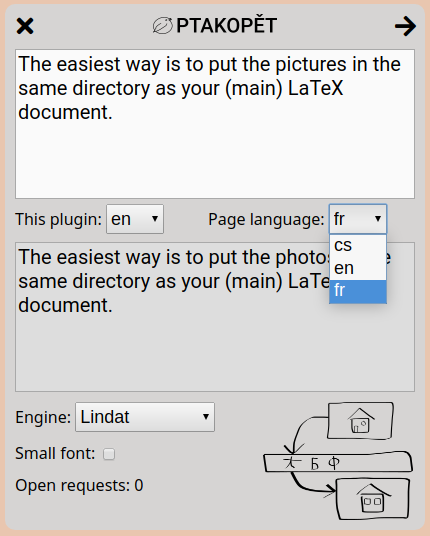
\includegraphics[width=0.6\textwidth]{img/ptakopet_old-1/lang_select}
    \caption{User interface of the \ptakopet{} old-1 browser extension}
    \label{fig:ptakopet_old-1/lang_select}
\end{figure}

The plugin shown in \cref{fig:ptakopet_old-1/lang_select}, contains two main textareas. The top one expected input in the language of the user. The bottom one eventually contained the backward translation. The translation was in the active input element (on the webpage). This process of three text elements (input, translation and backward translation) was hard to communicate to users, so the window also contained an explanatory diagram in the bottom right corner, as seen in \cref{fig:ptakopet_old-1/lang_select}.

The intended workflow was to write text to the top textarea and validate against the backward translation in the bottom one. During this process, the translated text appeared in the selected area on the web page. The active target input element was changed every time a possible element (all textareas and text inputs) got focus.

The plugin also contained other miscellaneous control elements, such as translator backend selector, small font checkbox and indicator of open requests. 

\begin{figure}[ht]
\centering
\begin{subfigure}{.5\textwidth}
  \centering
  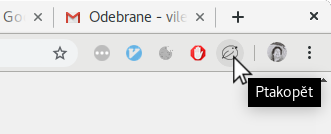
\includegraphics[width=.95\linewidth]{img/ptakopet_old-1/invoke_2}
  \caption{Toolbar icon}
  \label{fig:ptakopet_old-1/invoke_2}
\end{subfigure}%
\begin{subfigure}{.5\textwidth}
  \centering
  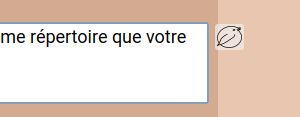
\includegraphics[width=.95\linewidth]{img/ptakopet_old-1/invoke_1}
  \caption{Input element icon}
  \label{fig:ptakopet_old-1/invoke_1}
\end{subfigure}
\caption{Two ways of launching \ptakopet{} old-1}
\label{}
\end{figure}

The \ptakopet{} window could be invoked in multiple ways: by clicking the toolbar button, as shown in \cref{fig:ptakopet_old-1/invoke_1}, by launching it from the context menu (right mouse button) or by clicking an icon, that appeared next to all web page text input elements.

\begin{figure}[ht]
    \centering
    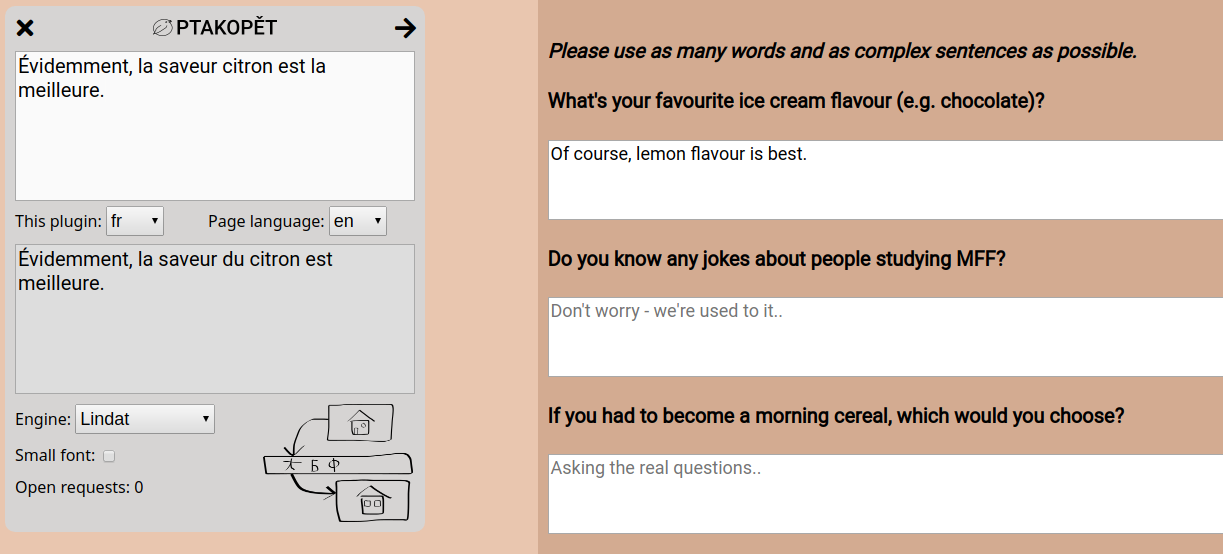
\includegraphics[width=1\textwidth]{img/ptakopet_old-1/ice_cream}
    \caption{\ptakopet{} helps a French-speaking user with filling in an English form}
    \label{fig:ptakopet_old-1/ice_cream}
\end{figure}

In \cref{fig:ptakopet_old-1/ice_cream}, the user selected the first web page input element, hence making it active to \ptakopet{} and wrote a text in their native language (French) to the first \ptakopet{} input. The backward translation removed a definite article for an uncountable noun; otherwise, the sentence matches the original. The English translation of the input sentence then appeared in the target textarea, as expected. Should the user now edit the English text, the translation would appear in the bottom \ptakopet{} textarea. Writing into the top \ptakopet{} input field would overwrite the manual changes, as hinted in the bottom right diagram in the \ptakopet{} window.

\pagebreak 

\subsection{Technical details}

\ptakopet{} old-1 was written entirely with basic HTML, CSS and JS stack with some usage of jQuery. There was no packaging or build system. Part of the codebase dealt with abstraction on top of different browser plugin APIs and the differences between content and background script execution. Most major browsers support the WebExtensions API of W3C, but there are some differences between browsers.

The rest of the code dealt with DOM manipulation and mostly with handling translation requests. Two translation backends were used: Khresmoi \citep{khresmoi} and LINDAT Translation \citep{popel-en-cs}, because of their ease of use and availability. At the time of deployment, LINDAT Translation supported translations between English, French, and Czech, while Khresmoi supported English, French, Czech, German, and Spanish.

Four months after the finished project was demoed, the API which \ptakopet{} used for communication with LINDAT Translation was deprecated and two months after that the Khresmoi translation service shut down. Instead of making necessary fixes, this project was abandoned for a newer version and the plugin was removed from the public listing.

\subsection{Conclusion}

This project was completed and met all criteria regarding quality and functionality, even though the extension was not usable on all websites, which stemmed from the extension architecture.

It was demoed during the Open Days at Charles University Faculty of Mathematics and Physics 2019, although only few visitors tried it. The demo page is not hosted publicly anymore, but source code is available.\footnotehref{https://github.com/zouharvi/ptakopet-old/tree/master/old-1/dod\_ufal}{github.com/zouharvi/ptakopet-old/tree/master/old-1/dod\_ufal} A part of the demo page is visible in \cref{fig:ptakopet_old-1/ice_cream}. The demo included a simple form with random personal questions in a foreign language, which visitors were to fill. The source language in the demo was Czech and, unfortunately, the foreign language was English, so it was hard to demonstrate the issue of outbound translation fully, as most people know English to at least some extent.

A four-page report was submitted.\footnotehref{https://github.com/zouharvi/ptakopet-old/blob/master/old-1/meta/report.pdf}{github.com/zouharvi/ptakopet-old/blob/master/old-1/meta/report.pdf} This first attempt for an outbound translation tool provided us with findings as what to avoid and what to focus on in the next version, \ptakopet{} old-2.

\section{\ptakopet{} old-2}

\subsection{Introduction}

The second version of \ptakopet{} aimed to extend the functionality of the first version, while improving on usability. One of the downsides of the \ptakopet{} old-1 was the disunified behaviour and lack of consistency across different websites. The user interface proved to be too complex to work with and hence we opted for a more traditional approach. The entire application would then be hosted on a separate web page with no interaction with other web pages. This form of serving public machine translation is similar to the one by Google, Microsoft, DeepL and other online services.

In addition to the major change of moving from browser plugin to a standalone web page, we decided to add visual quality estimation cues in the form of word highlighting (from word-level quality estimation models).

\ptakopet{} old-2 was created to meet the requirements of class Semestral Project and has a corresponding specification document.\footnotehref{https://github.com/zouharvi/ptakopet-old/blob/master/old-2/meta/Ptakop\%C4\%9Bt\%20v2\%20-\%20specification.pdf}{github.com/ zouharvi/ ptakopet-old/ blob/ master/ old-2/ meta/ \ptakopet{} v2 - specification.pdf} It was again supervised by Ondřej Bojar.

\subsection{Usage}

There are generally two use cases for the second version: Outbound translation and user translation quality estimation.

\subsubsection*{Outbound translation}

In outbound translation the user tries to translate text to and validate produced translation in a language their are not familiar with.

To perform outbound translation, the user selects the source and target languages from the select box, then writes text in the source language input window (first textarea in \cref{fig:ptakopet_old-2/john_screen}). Problematic words in the source and target text can be seen (more intense colouring means worse quality; purple signifies, that the particular word was not translated) as well as backward translation of the already translated text (third textarea in \cref{fig:ptakopet_old-2/john_screen}).

\begin{figure}[ht]
    \centering
    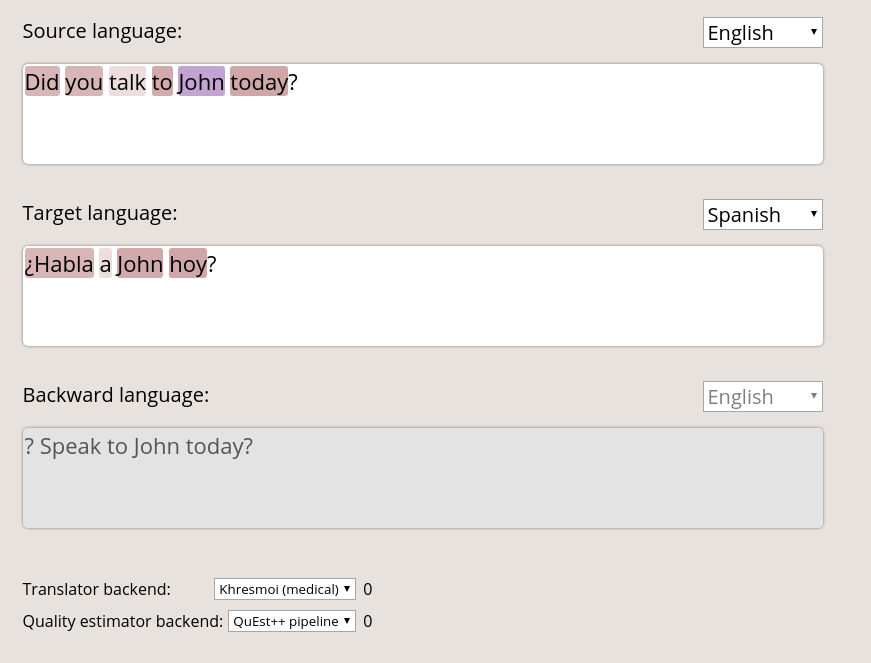
\includegraphics[width=0.85\textwidth]{img/ptakopet_old-2/john_screen}
    \caption{Example usage of \ptakopet{} old-2. The more red the word highlighting, the worse the estimated translation quality. Purple highlighting was used for words, which were not translated.}
    \label{fig:ptakopet_old-2/john_screen}
\end{figure}

\subsubsection*{User translation quality estimation}

The user could then follow up from the previous use case with a more agile workflow and dynamically edit the translated text. They would see the quality estimation of their own translation, as well as backward translation.

In this case the quality estimation is not exactly the same as the task defined by WMT, because the provided translation is not a product of an MT system, but of a human user. With current QE models we do not think that this can be used reliably.

\subsection{Technical details}

The second version was also written in plain HTML, CSS, JS + jQuery (frontend) and Python 3 (backend request handler), but contains many interactions (through system pipes) to other frameworks written in Python 2, Java, Perl and C++. The frontend tech stack is used contrary to modern approaches to web development, but the limited scale of this project and focus on other aspects allowed for it.

The backend ran at servers provided by ÚFAL and responded to requests for either quality estimation or word alignment. The same two translation backends were used: Khresmoi \citep{khresmoi} and LINDAT Translation \citep{popel-en-cs}.

\subsubsection*{Quality Estimation}

There were two quality estimation backends: DeepQuest for English-German and QuEst++ for English-Spanish. 
% The user could select a language pair not compatible with the selected quality estimator, but the result would not be useful, except for their translation quality estimation.

Highlighting parts of texts seems trivial at first, but taking into consideration, that the text must be editable and that the highlighting must work on different zoom levels, browsers and on mobile, it soon becomes complex.
Finally, we opted for a jQuery plugin developed originally by Will Boyd,\footnotehref{https://github.com/lonekorean/highlight-within-textarea}{github.com/lonekorean/highlight-within-textarea} which we forked,\footnotehref{https://github.com/zouharvi/highlight-within-textarea}{github.com/zouharvi/highlight-within-textarea} as some changes to the internal workings of this plugin were necessary.
% (dynamic style attribute instead of based on classes)
We also wanted to highlight words, which were not translated. To do this, we highlighted all words, which were mapped via alignment to a word of the same form. Such an occurrence is displayed in \cref{fig:ptakopet_old-2/john_screen}.

\subsubsection*{Alignment}

Fast align\footnotehref{https://github.com/clab/fast\_align}{github.com/clab/fast\_align} was used for the alignment backend, as it was recommended in the QuEst++ documentation. Word alignment was necessary for the highlighting itself as well as for QuEst++.

\subsection{Issues}

We later found that we used Fast align incorrectly, applying the unsupervised word-alignment method only to the single input sentence pair given. Since the model lacks any lexical knowledge, it thus essentially provided a simple diagonal alignment most of the time.

Because of missing Access-Control-Allow-Origin header on the Khresmoi translator backend, a proxy was added. This was unavoidable but a wrong decision since it is considered unsafe and software such as Avast would notify the users.

At the time of the deployment, the web hosting server had a valid SSL certificate but made requests to unsafe servers, so it had to be served over HTTP.

Another issue was the lack of a clear indication of supported language pairs. \ptakopet{} allowed users to use a quality estimation model even for language pairs that the model did not support.

Setting up the server was also a difficult task, as proper replicable setup scripts were not written.

\subsection{Conclusion}

While \ptakopet{} old-2 passed as a semestral project, there were many ideas on how to improve the experience and project quality. In \ptakopet{} old-2 only English-Spanish and English-German language pairs were supported by QuEst++ and DeepQuest respectively. Especially DeepQuest could be used with more language pairs if relevant data were provided. DeepQuest also reported only binary values \texttt{OK} or \texttt{BAD} at that time, but continuous confidence values from 0 to 1 existed inside. Extracting them would have provided more information to the user.

During development, the whole project accumulated significant technical debt. This was due to decisions such as writing in JavaScript without a framework, not having more structured backend and missing setup scripts.

Both technical and user documentation\footnotehref{https://ptakopet.vilda.net/docs/old-2}{ptakopet.vilda.net/docs/old-2} was written on this version.

\newpage

\section{Industry} \label{sec:related_industry}

As far as we observed, modern outbound translation workflow is condensed to roundtrip translation done manually by users (switching the language direction and copy-pasting the translated text).

Quality estimation is used in translation companies mostly to minimize post-editing costs. Despite that, QE cues are missing in most of the mainstream public translation services, such as Google Translate\footnotehref{https://translate.google.com/}{translate.google.com} (provides alternatives to words and shows their usage frequencies), Microsoft Bing Translator\footnotehref{https://www.bing.com/translator}{bing.com/translator} or DeepL\footnotehref{https://www.deepl.com/en/translator}{deepl.com/en/translator} (provides alternatives to phrases).

\subsubsection{Memsource}

The company Memsource, which specializes in cloud-based translation environment with tools like translation memory and terminology management, is also deploying quality estimation models, to minimize post-editing cost. For example, if a machine-translated sentence receives a full score, then there is no need to pay professional human translators to verify the translation. Even though they are developing their models in-house and closed-source, they disclosed some details in one of their blog posts.\footnotehref{https://www.memsource.com/blog/2018/10/01/machine-translation-quality-estimation-memsources-latest-ai-powered-feature/}{memsource.com/blog/2018/10/01/machine-translation-quality-estimation-memsources-latest-ai-powered-feature/}

Notable is their way of presenting the quality estimation data. Instead of displaying the percentage score in any form (e.g. highlighting), they approach this as a classification problem with the classes: $100\%$: probably perfect translation, $95\%$: possibly requires minor post-editing, $85\%$: will require post-editing, no score: needs to be manually checked. They focus on the phrase-level and sentence-level quality estimation.

\subsubsection{Unbabel}

The company Unbabel, which delivers machine translation solutions, is also developing\footnotehref{https://unbabel.com/blog/unbabel-translation-quality-systems/}{unbabel.com/blog/unbabel-translation-quality-systems/} a QE pipeline. As opposed to Memsource, most of their QE research is public, such as \cite{martins-unbabel:2016} and \cite{openkiwi}. They also make use of both word-level and phrase-level quality estimation. One of their components, OpenKiwi, is also part of \ptakopet{} and is described in \cref{subsec:openkiwi}.